\documentclass[LPSC_Labo03_SDeriaz]{subfiles}


\begin{document}
\section{Conclusion}
Le but principal du laboratoire a été atteint (loop avec affichage de la fractale) et un objectif secondaire a été réalisé : l'implémentation sous forme de pipeline. Un zoom "dynamique" a également été réalisé afin de démontrer la vitesse de calcul du pipeline. Il faut noter toutefois que la vitesse du zoom (10 rapprochements par seconde) est toujours bien en dessous de la fréquence de rafraichissement du pipeline (82 images par seconde). Cette fréquence pourrait d'ailleurs être augmentée en ajustant plus finement la fréquence de fonctionnement. À ce jour la fréquence à été fixée arbitrairement à \SI{50}{\mega\hertz} pour respecter les contraintes de timing.
\subsection{Utilisation du FPGA}
\subsubsection{Méthode loop}
\begin{figure}[H]
\centering
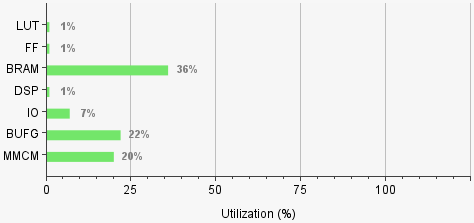
\includegraphics[scale=0.5]{utilisation_graph_loop.png}
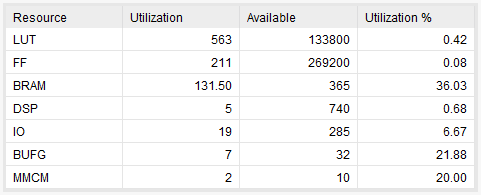
\includegraphics[scale=0.5]{utilisation_table_loop.png}
\caption{Graph et table d'utilisation du FPGA fourni par Vivado}
\end{figure}
L'utilisation des BRAM est importante et l'implémentation de l'itérateur a nécessité 5 DSP
\subsubsection{Méthode pipeline}
\begin{figure}[H]
\centering
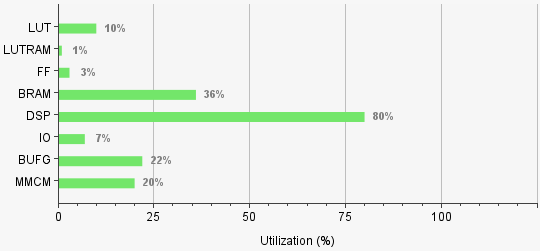
\includegraphics[scale=0.5]{utilisation_graph_pipeline.png}
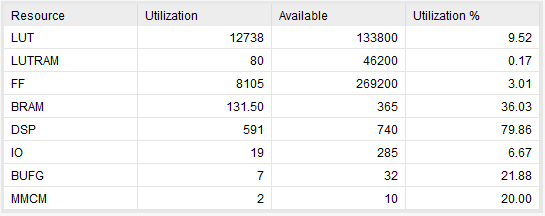
\includegraphics[scale=0.5]{utilisation_table_pipeline.png}
\caption{Graph et table d'utilisation du FPGA fourni par Vivado}
\end{figure}
L'utilisation des DSP est très importante, ce qui est attendu car on en attend environ 100x plus qu'avec la version loop. L'utilisation des BRAM est identique car la mémoire vidéo est la même.
\end{document}